% Copyright (c)  2005-2010 EDF-EADS-PHIMECA.
% Permission is granted to copy, distribute and/or modify this document
% under the terms of the GNU Free Documentation License, Version 1.2
% or any later version published by the Free Software Foundation;
% with no Invariant Sections, no Front-Cover Texts, and no Back-Cover
% Texts.  A copy of the license is included in the section entitled "GNU
% Free Documentation License".
\renewcommand{\filename}{docUC_MinMax_DetExperimentPlane.tex}
\renewcommand{\filetitle}{UC : Creation of a deterministic experiment plane : Axial, Box, Composite, Factorial patterns}

% \HeaderNNIILevel
% \HeaderIILevel
\HeaderIIILevel

\label{determExpPlane}



\index{Experiment Plane!Factorial scheme}
\index{Experiment Plane!Composite scheme}
\index{Experiment Plane!Axial scheme}
\index{Experiment Plane!Box scheme}
\index{Experiment Plane!Scaling}
\index{Experiment Plane!Translation}

The objective of this Use Case is to create an experiment plane which scheme is specified and then denoted {\itshape deterministic} experiment plane.\\


Details on experiment planes  may be found in the Reference Guide (\href{OpenTURNS_ReferenceGuide.pdf}{see files Reference Guide - Step C -- Min-Max approach using Experiment Planes}).\\

Details on each object may be found in the User Manual  (\href{OpenTURNS_UserManual_TUI.pdf}{see User Manual - Experiment Planes / Stratified Experiment Planes}).\\


Open TURNS enables to define four types of deterministic experiment planes : axial, composite, factorial and box.\\

In order to define an experiment plane, follow the 3  steps, whatever the type of the experiment plane, where $n$ is the dimension of the space and $n_{level}$ the number of levels (the same for each direction except for the Box grid) :
\begin{itemize}
\item Step 1 : Define a reduced and centered grid structure, centered on $\vect{0} \in \mathbb{R}^n$, by specifying the levels which will be consider on each direction,
\item Step 2 : Scale each direction with a specific scale factor for each direction, in order to give a unit effect on each direction,
\item Step 3 : Translate the scaled grid structure onto a specified center point.
\end{itemize}

Each experiment plane has a specific method to define its reduced and centered grid structure :
\begin{itemize}
\item {\bf Axial} : the  points grid is obtained by discretizing each direction according to the specified levels, symmetrically with respect to 0. The number of points generated is $1 + 2n* n_{level}$.
\item {\bf Factorial} : the  points grid is obtained by discretizing each principal diagonal according to the specified levels, symmetrically with respect to 0. The number of points generated is $1 +  2^n*n_{level}$.
\item {\bf Composite} : the  points grid is obtained as the union between an axial and a factorial experiment plane. The number of points generated is $1 + 2n*n_{level} +  2^n*n_{level}$.
\item {\bf Box} : the  points grid is obtained by regularly discretizing the unit pavement $[0, 1]^n$, with the number of intermediate points specified for each direction.  The number of points generated is $\displaystyle \prod_{i=1}^{n} (2+n_{level}(direction \, \, i))$.
\end{itemize}

In order to scale each direction according to a specified factor or/and to translate the points grid until a specified center, the methods {\itshape scale} and {\itshape translate} must be used.\\

The following example works in $\mathbb{R}^2$.\\

\requirements{
  \begin{description}
  \item[$\bullet$] none
  \end{description}
}
{
  \begin{description}
  \item[$\bullet$] a centered and reducted grid structure : {\itshape myCenteredReductedPlane}
  \item[type:] ExperimentPlane, which type is Axial, Composite, Factorial or Box
  \item[$\bullet$] the numerical sample associated to the centered and reducted grid structure then scaled then translated grid structure : {\itshape mySample}
  \item[type:] NumericalSample
  \end{description}
}

\textspace\\
Python script for this UseCase :


\begin{lstlisting}

  # Define a scale factor for each direction
  scaledVector = NumericalPoint( (1.5, 2.5) )

  # Define the translation until the final center of the experiment plane
  translationVector = NumericalPoint( (2., 3.) )

  # Define the different levels of the grid structure
  # CARE : for the axial, composite and factorial experiment planes,
  # these levels are all applied along each direction
  # Here : 3 levels on each direction
  levels = NumericalPoint( (1., 1.5, 3.) )

  # For the box experiment plane, levels specifies the number of
  # intermediate points on each direction (one per direction)
  # Here : direction 1 will be discretized with 2 intermediate points
  # and direction 2 with 4 intermediate points
  levelsBox = NumericalPoint( (2., 4.) )


  # STEP 1 : Define a reduced and centered grid structure

  # AXIAL structure
  myCenteredReductedGrid = Axial(2,levels)

  # COMPOSITE structure
  myCenteredReductedGrid = Composite(2,levels)

  # FACTORIAL structure
  myCenteredReductedGrid = Factorial(2,levels)

  # BOX structure
  myCenteredReductedGrid = Box(levelsBox)

  # Generate the numerical sample (centered and reducted grid structure)
  # a NumericalSample is created
  mySample = myCenteredReductedGrid.generate()

  # Get the number of points of the centered and reducted grid structure
  pointsNumber = mySample.getSize()


  # STEP 2 : Scale each direction with a specific scale factor

  # The NumericalSample is transformed
  mySample.scale(scaledVector)


  # STEP 3 : Translate the scaled grid structure onto a specified center point

  # The NumericalSample is transformed
  mySample.translate(translationVector)

  # Print the numerical sample
  print mySample
\end{lstlisting}
\textspace\\


Figures \ref{AxialGrid} to \ref{TranslatedScaledBoxGrid} draw the different grid structures obtained after the {\itshape scale} or {\itshape translate} methods.

\begin{figure}[H]
  \begin{minipage}{10cm}
    \begin{center}
      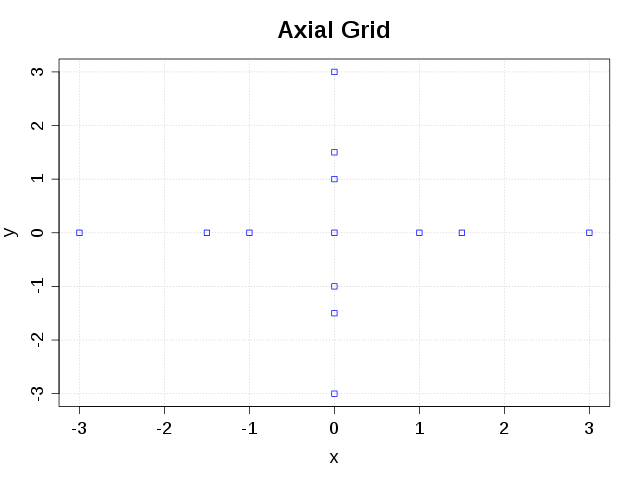
\includegraphics[width=8cm]{AxialGrid.png}
      \caption{Axial Experiment Plane : initial grid.}
      \label{AxialGrid}
    \end{center}
  \end{minipage}
  \hfill
  \begin{minipage}{10cm}
    \begin{center}
      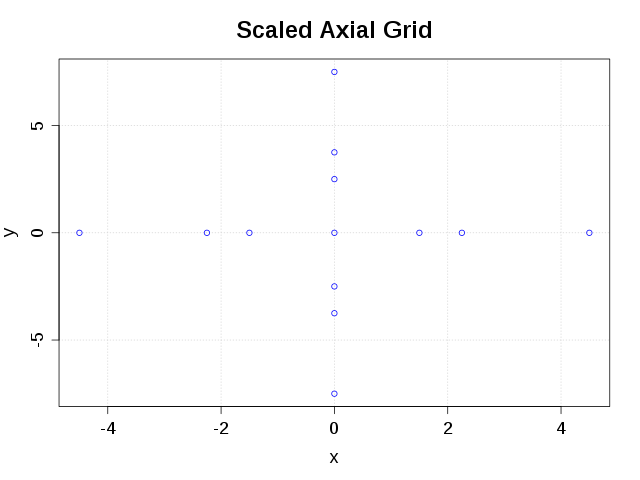
\includegraphics[width=8cm]{ScaledAxialGrid.png}
      \caption{Axial Experiment Plane : after scaling.}
      \label{ScaledAxialGrid}
    \end{center}
  \end{minipage}
\end{figure}

\begin{figure}[H]
  \begin{center}
    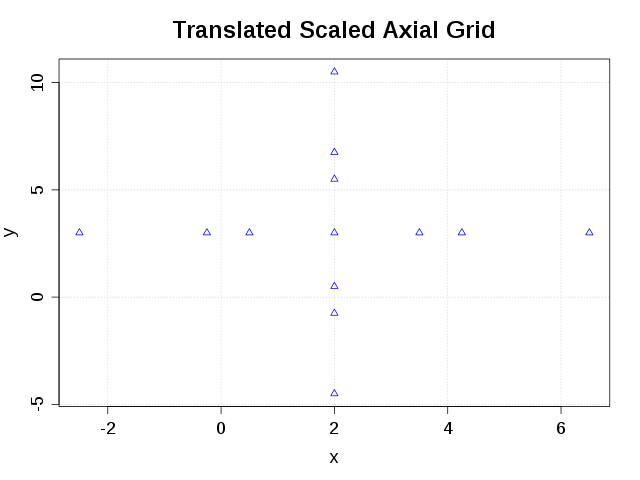
\includegraphics[width=8cm]{TranslatedScaledAxialGrid.png}
  \end{center}
  \caption{Axial Experiment Plane : after scaling and translation.}
  \label{TranslatedScaledAxialGrid}
\end{figure}



\begin{figure}[H]
  \begin{minipage}{10cm}
    \begin{center}
      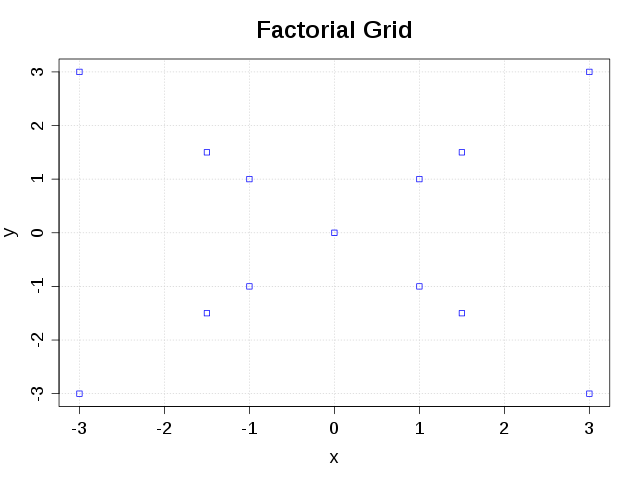
\includegraphics[width=8cm]{FactorialGrid.png}
      \caption{Factorial Experiment Plane : initial grid.}
      \label{FactorialGrid}
    \end{center}
  \end{minipage}
  \hfill
  \begin{minipage}{10cm}
    \begin{center}
      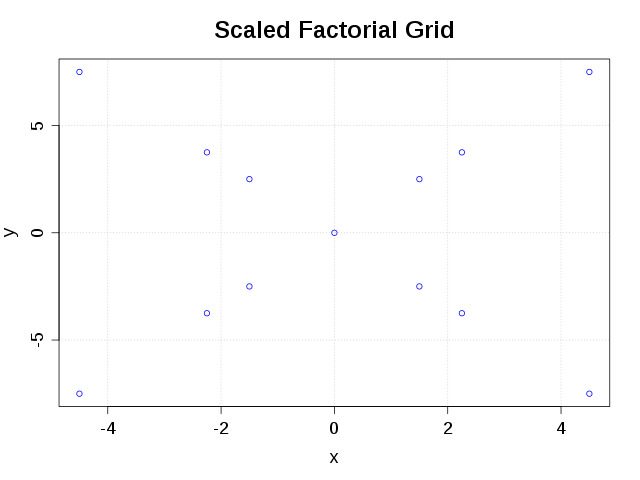
\includegraphics[width=8cm]{ScaledFactorialGrid.png}
      \caption{Factorial Experiment Plane : after scaling.}
      \label{ScaledFactorialGrid}
    \end{center}
  \end{minipage}
\end{figure}




\begin{figure}[H]
  \begin{center}
    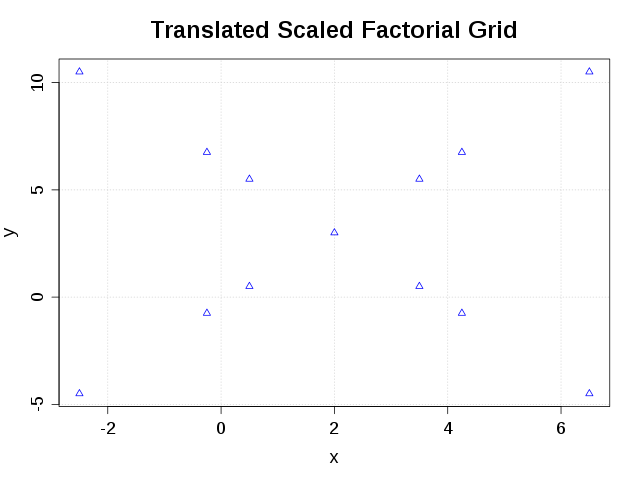
\includegraphics[width=8cm]{TranslatedScaledFactorialGrid.png}
  \end{center}
  \caption{Factorial Experiment Plane : after scaling and translation.}
  \label{TranslatedScaledFactorialGrid}
\end{figure}





\begin{figure}[H]
  \begin{minipage}{10cm}
    \begin{center}
      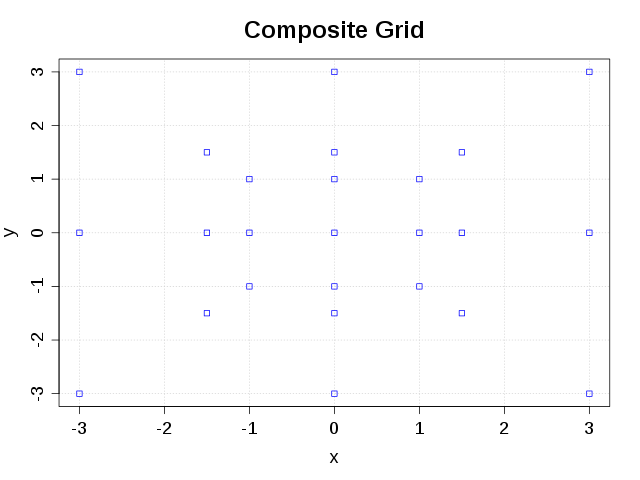
\includegraphics[width=8cm]{CompositeGrid.png}
      \caption{Composite Experiment Plane : initial grid.}
      \label{CompositeGrid}
    \end{center}
  \end{minipage}
  \hfill
  \begin{minipage}{10cm}
    \begin{center}
      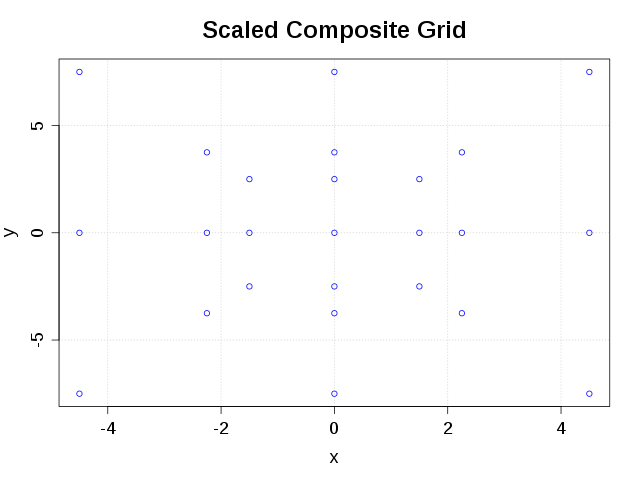
\includegraphics[width=8cm]{ScaledCompositeGrid.png}
      \caption{Composite Experiment Plane : after scaling.}
      \label{ScaledCompositeGrid}
    \end{center}
  \end{minipage}
\end{figure}

\begin{figure}[H]
  \begin{center}
    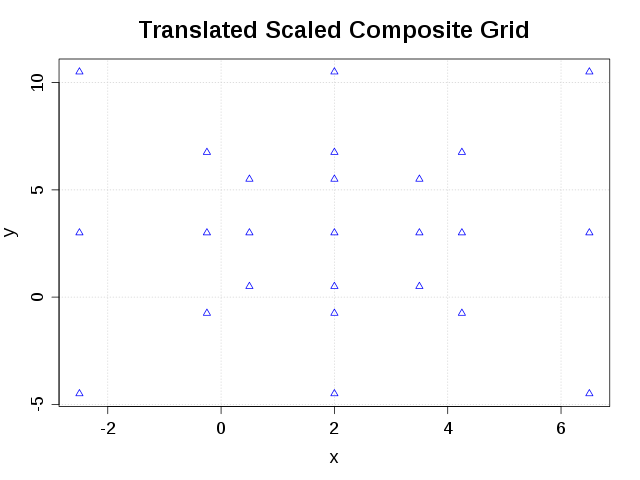
\includegraphics[width=8cm]{TranslatedScaledCompositeGrid.png}
  \end{center}
  \caption{Composite Experiment Plane : after scaling and translation.}
  \label{TranslatedScaledCompositeGrid}
\end{figure}


\begin{figure}[H]
  \begin{minipage}{10cm}
    \begin{center}
      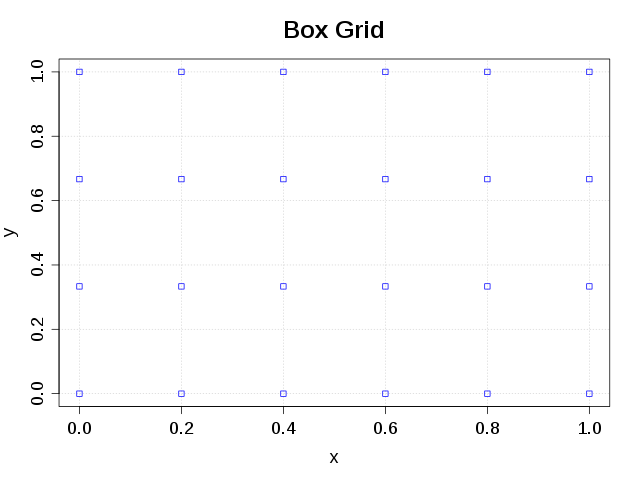
\includegraphics[width=8cm]{BoxGrid.png}
      \caption{Box Experiment Plane : initial grid.}
      \label{BoxGrid}
    \end{center}
  \end{minipage}
  \hfill
  \begin{minipage}{10cm}
    \begin{center}
      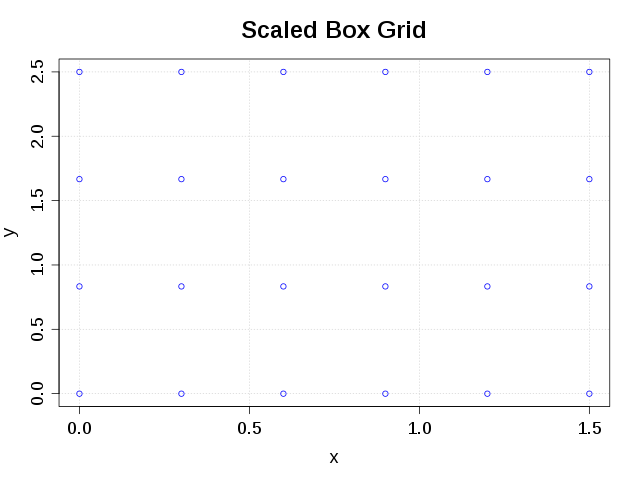
\includegraphics[width=8cm]{ScaledBoxGrid.png}
      \caption{Box Experiment Plane : after scaling.}
      \label{ScaledBoxGrid}
    \end{center}
  \end{minipage}
\end{figure}

\begin{figure}[H]
  \begin{center}
    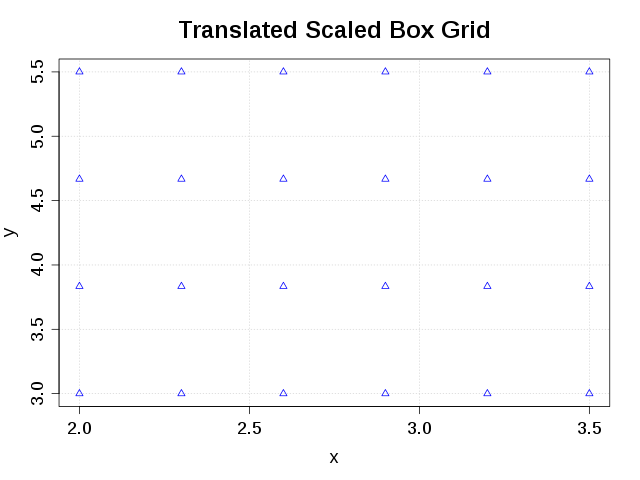
\includegraphics[width=8cm]{TranslatedScaledBoxGrid.png}
  \end{center}
  \caption{Box Experiment Plane : after scaling and translation.}
  \label{TranslatedScaledBoxGrid}
\end{figure}




